%%%%%%%%%%%%%%%%%%%%%%%%%%%%%%%%%%%%%%%%%%%%%%%%%%%%%%%%%%%%%%%%%%%%%
% In English:
%    This is a Latex template for São Paulo Research Foudation (FAPESP)
%         reports (annual or final).
%    This is the modified version of the original Latex template from
%         following website.
%    Original Source: http://www.howtotex.com
%    For information about FAPESP, check http://www.fapesp.br/en
%    This template targets mainly on reports in Portuguese language.
%    New additions and changes in the latest version:
%        - Added the possibility of including multiple members in the 
%          research team, with the commands \memberA{Name of Member A} 
%          \memberB{Name of Member B} \memberC{Name of Member C} etc.
%        - Included commands to define project modality and the research 
%          agency (if you want to use the same model for other research 
%          agencies such as CAPES, CNPq etc).
%
% In Portuguese:
%    Este é um modelo Latex para relatórios (anual ou final) da Fundação 
%         de Amparo à pesquisa do Estado de São Paulo (FAPESP).
%    Esta é uma versão modificada do modelo Latex do site supra mencionado.
%    Para informações sobre a FAPESP, verifique http://www.fapesp.br
%    Esse modelo foca principalmente nos relatórios escritos em Português.
%    Novas adições e alterações na última versão:
%       - Foi adicionada a possibilidade de incluir vários membros no 
%         grupo de pesquisas, com os comandos \membroA{Nome do Membro A} 
%         \membroB{} \membroC{} etc.
%       - Foram incluídos comandos para definir modalidade de projeto e
%         agência de fomento (caso queira utilizar o mesmo modelo para 
%         outras agências, CAPES, CNPq etc).
%
% Author/Autor: André Leon Sampaio Gradvohl, Dr.
% Email:        andre.gradvohl@gmail.com
% Lattes CV:    http://lattes.cnpq.br/9343261628675642
% GitHub: http://gradvohl.github.io/
% 
% Last update/Última versão: 19/Feb/2018
%
%%%%%%%%%%%%%%%%%%%%%%%%%%%%%%%%%%%%%%%%%%%%%%%%%%%%%%%%%%%%%%%%%%%%%%
\documentclass[12pt]{report}
\usepackage[a4paper]{geometry}
\usepackage[utf8]{inputenc}
\usepackage[english,portuguese]{babel}
\usepackage[myheadings]{fullpage}
\usepackage[T1]{fontenc}
\usepackage{fancyhdr}
\usepackage{graphicx, setspace}
\usepackage{sectsty}
\usepackage{url}
\usepackage{pdfpages}
\usepackage{subcaption}
\usepackage{amsmath}
\usepackage{multirow}
\usepackage{tikz}
\usepackage{minted}
\usepackage{hyperref}
\def\checkmark{\tikz\fill[scale=0.4](0,.35) -- (.25,0) -- (1,.7) -- (.25,.15) -- cycle;}

\DeclareMathOperator{\diag}{diag}
\DeclareMathOperator{\ai}{Ai}
\DeclareMathOperator{\re}{Re}
\DeclareMathOperator{\im}{Im}
\DeclareMathOperator{\ee}{\rm e}
\DeclareMathOperator{\supp}{supp}
\renewcommand{\Re}{\mathop{\rm Re}}
\newcommand{\res}{\mathop{\rm Res}}
\renewcommand{\Im}{\mathop{\rm Im}}
\newcommand{\N}{\mathbb{N}}
\newcommand{\C}{\mathbb{C}}
\newcommand{\R}{\mathbb{R}}
\newcommand{\Z}{\mathbb{Z}}
\newcommand{\D}{\mathbb{D}}
\newcommand{\Q}{\mathbb{Q}}
\newcommand{\E}{\mathbb{E}}
\newcommand{\boh}{\mathit{o}}
\newcommand{\Boh}{\mathcal{O}}
\newcommand{\bbp}{\bm K_{\mathrm{BBP}}}
\newcommand{\ii}{\mathrm{i}}
\newcommand{\dd}{\mathrm{d}}
\newcommand*{\deff}{\mathrel{\vcenter{\baselineskip0.5ex \lineskiplimit0pt
			\hbox{\scriptsize.}\hbox{\scriptsize.}}}%
	=}
\newcommand*{\revdeff}{=\mathrel{\vcenter{\baselineskip0.5ex \lineskiplimit0pt
			\hbox{\scriptsize.}\hbox{\scriptsize.}}}%
}
%%------ 
%% Comandos gerais
%% Observação: o arquivo "comandos.tex" tem que estar presente.
%%------
%%%%%%%%%%%%%%%%%%%%%%%%%%%%%%%%%%%%%%%%%%%%%%%%%%%%%%%%%%%%%%%%%%%%%
% In English:
%    This is a list of commands specification for FAPESP reports.
%
% In Portuguese:
%    Esta é uma lista de especificação de comandos para relatórios
% da Fundação de Amparo à pesquisa do Estado de São Paulo (FAPESP).
%
% Author/Autor: André Leon Sampaio Gradvohl, Dr.
% Email:        andre.gradvohl@gmail.com
% Lattes CV:    http://lattes.cnpq.br/9343261628675642
% 
% Last update/Última versão: 11/Sep/2016
%%%%%%%%%%%%%%%%%%%%%%%%%%%%%%%%%%%%%%%%%%%%%%%%%%%%%%%%%%%%%%%%%%%%%%

\def\checkmark{\tikz\fill[scale=0.4](0,.35) -- (.25,0) -- (1,.7) -- (.25,.15) -- cycle;}

\DeclareMathOperator{\diag}{diag}
\DeclareMathOperator{\ai}{Ai}
\DeclareMathOperator{\re}{Re}
\DeclareMathOperator{\im}{Im}
\DeclareMathOperator{\ee}{\rm e}
\DeclareMathOperator{\supp}{supp}
\renewcommand{\Re}{\mathop{\rm Re}}
\newcommand{\res}{\mathop{\rm Res}}
\renewcommand{\Im}{\mathop{\rm Im}}
\newcommand{\N}{\mathbb{N}}
\newcommand{\C}{\mathbb{C}}
\DeclareMathOperator{\Tr}{Tr}
\newcommand{\R}{\mathbb{R}}
\newcommand{\Z}{\mathbb{Z}}
\newcommand{\D}{\mathbb{D}}
\newcommand{\Q}{\mathbb{Q}}
\newcommand{\boh}{\mathit{o}}
\newcommand{\Boh}{\mathcal{O}}
\newcommand{\bbp}{\bm K_{\mathrm{BBP}}}
\newcommand{\ii}{\mathrm{i}}
\newcommand{\dd}{\mathrm{d}}
\newcommand*{\deff}{\mathrel{\vcenter{\baselineskip0.5ex \lineskiplimit0pt
			\hbox{\scriptsize.}\hbox{\scriptsize.}}}%
	=}
\newcommand*{\revdeff}{=\mathrel{\vcenter{\baselineskip0.5ex \lineskiplimit0pt
			\hbox{\scriptsize.}\hbox{\scriptsize.}}}%
}

\newcommand{\HRule}[1]{\rule{\linewidth}{#1}}
\setcounter{tocdepth}{3}
\setcounter{secnumdepth}{3}

\newcommand{\titulo}[1]{\def\meuTitulo{#1}}
\newcommand{\tituloIngles}[1]{\def\meuTituloIngles{#1}}
\newcommand{\numProjeto}[1]{\def\numFAP{#1}}
\newcommand{\tipoRelatorio}[1]{\def\tipoRelat{#1 }} %o espaço depois do #1 é importante
\newcommand{\modalidadeProjeto}[1]{\def\modProjeto{#1}} 
\newcommand{\agFomento}[2]{\def\agFom{#1} \def\siglaAgFom{#2}} %extenso Sigla
\newcommand{\autor}[1]{\def\nomeAutor{#1}}
\newcommand{\cidade}[1]{\def\nomeCidade{#1}}
\newcommand{\universidade}[1]{\def\nomeUniversidade{#1}}
\newcommand{\faculdade}[1]{\def\nomeFaculdade{#1}}
\newcommand{\periodoVigencia}[1]{\def\periodVig{#1}}
\newcommand{\periodoRelatorio}[1]{\def\periodRelat{#1}}

\author{}
\date{}

%Definição de membros da equipe de pesquisas
\newcommand{\membroA}[1]{\def\nomeMembroA{#1}}
\newcommand{\membroB}[1]{\def\nomeMembroB{#1}}
\newcommand{\membroC}[1]{\def\nomeMembroC{#1}}
\newcommand{\membroD}[1]{\def\nomeMembroD{#1}}
\newcommand{\membroE}[1]{\def\nomeMembroE{#1}}
\newcommand{\membroF}[1]{\def\nomeMembroF{#1}}

\newcommand{\Figure}[1]{Figura~\ref{fig:#1}}
\newcommand{\Table}[1] {Tabela~\ref{#1}}
\newcommand{\Equation}[1] {Equa\c{c}\~ao~\ref{#1}}
\newcommand{\addFigure}[3] { %Parametros scale, fig_name, caption 
    \begin{figure}[!hbt]
      \centering
      \includegraphics[scale=#1]{figures/}
      \caption{#3}\label{fig:#2}
    \end{figure}
}

\newcommand{\geraTitulo}{
\clearpage
\begin{titlepage}
  \begin{center}
      \vspace*{-3cm}
       { \setstretch{.5} 
         \textsc{\nomeUniversidade} \\
         \HRule{.2pt}\\
         \textsc{\nomeFaculdade}
       }

       \vspace{5.5cm}

       \Large \textbf{\textsc{\meuTitulo}}
 	  \HRule{1.5pt} \\ [0.5cm]
       \linespread{1}
       \large Relatório Científico 
       \ifdefined\tipoRelat
            \tipoRelat
       \fi
       do projeto 
       \ifdefined\modProjeto
           na modalidade \modProjeto,
       \fi
       fomentado pela \agFom. \\ 
   	   \HRule{1.5pt} \\ [0.5cm]

       \ifdefined\numFAP
          Projeto \siglaAgFom~\texttt{\#\numFAP}
          \\ [0.5cm]
       \fi
        Pesquisador Responsável: \nomeAutor
        
        \hspace{2cm}
        
        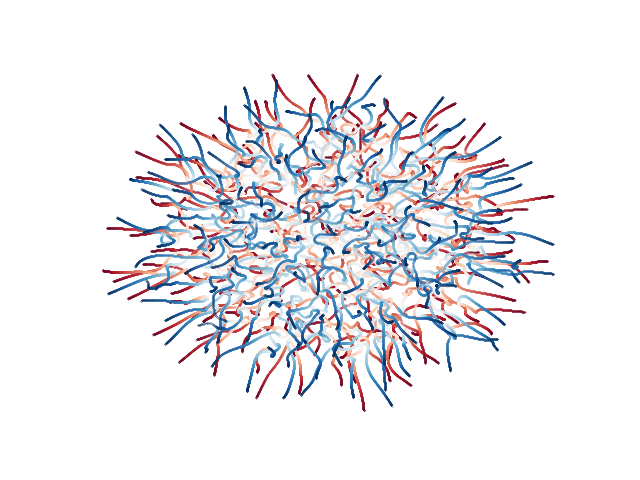
\includegraphics[scale=0.7]{Assets/CuteCircleWhite}
       
        \vfill
       
        {\normalsize  \nomeCidade, \today}
 \end{center}
 \end{titlepage}
}

\usepackage{titlesec}
\titleformat{\chapter}{\normalfont\LARGE\bfseries}{\thechapter}{1em}{}
\titlespacing*{\chapter}{0pt}{3.5ex plus 1ex minus .2ex}{2.3ex plus .2ex}

%----------------------------------------------------------------------
% Cabeçalho e rodapé
%----------------------------------------------------------------------
\pagestyle{fancy}
\fancyhf{} % Limpa todos os campos de header and footer fields
\renewcommand{\headrulewidth}{0pt}
\fancyfoot[R]{\thepage}

\addto\captionsportuguese{\renewcommand{\contentsname}{Sumário}}
\addto\captionsportuguese{\renewcommand{\bibname}{Referências Bibliográficas}}

%------
% Resumo e Abstract
%------
\newcommand{\Resumo}[1]{
   \begin{otherlanguage}{portuguese}
       \addcontentsline{toc}{chapter}{Resumo}
       \begin{abstract} \thispagestyle{plain} \setcounter{page}{2}
          #1
        \end{abstract}
   \end{otherlanguage} 
} %end \Resumo

\newcommand{\Abstract}[1]{
   \begin{otherlanguage}{english}
      \addcontentsline{toc}{chapter}{Abstract}
      \begin{abstract} \thispagestyle{plain} \setcounter{page}{3}
       #1
      \end{abstract}    
    \end{otherlanguage} 
} %end \abstract

%------
% Folha de rosto
%------
\newcommand{\folhaDeRosto}{
   \chapter*{Informações Gerais do Projeto}
   \addcontentsline{toc}{chapter}{Informações Gerais do Projeto}
   \begin{itemize}
      \item Título do projeto: 
            \begin{itemize}\item[] \textbf{\meuTitulo} \end{itemize}
      \item Nome do pesquisador responsável: 
            \begin{itemize}\item[]\textbf{\nomeAutor}\end{itemize}
      \item Instituição sede do projeto: 
            \begin{itemize}
               \item[]\textbf{\nomeFaculdade \ da \nomeUniversidade} 
            \end{itemize}
      \item Equipe de pesquisa:
            \begin{itemize}
               \ifdefined\nomeMembroA
                 \item[]\textbf{\nomeMembroA}
               \else 
                 \item[]\textbf{\nomeAutor}
               \fi
               \ifx\nomeMembroB\undefined\else \item[]\textbf{\nomeMembroB}\fi
               \ifx\nomeMembroC\undefined\else \item[]\textbf{\nomeMembroC}\fi
               \ifx\nomeMembroD\undefined\else \item[]\textbf{\nomeMembroD}\fi
               \ifx\nomeMembroE\undefined\else \item[]\textbf{\nomeMembroE}\fi
               \ifx\nomeMembroF\undefined\else \item[]\textbf{\nomeMembroF}\fi
             \end{itemize}
       
          \ifdefined \numFAP
             \item Número do projeto de pesquisa:
             \begin{itemize}
                 \item[]\textbf{\numFAP} 
             \end{itemize}
          \fi  
       \item Período de vigência:
            \begin{itemize}
               \item[]\textbf{\periodRelat} 
            \end{itemize}
       \item Período coberto por este relatório científico:
            \begin{itemize}
               \item[]\textbf{\periodVig} 
            \end{itemize}
   \end{itemize}
   \clearpage
}


\newcommand\underrel[2]{\mathrel{\mathop{#2}\limits_{#1}}}

\newcommand{\matriz}[1]{\hat#1}

\newcommand{\many}[2]{$#1_1, #1_2, \dots, #1_#2$}

\newcommand{\cmany}[3]{$#1_1 #3 #1_2 #3 \dots #3 #1_#2$}

\newcommand{\mmany}[2]{ #1_1, #1_2, \dots, #1_#2 }

\newcommand{\mcmany}[3]{#1_1 #3 #1_2 #3 \dots #3 #1_#2}

\newcommand{\set}[1]{\{#1\}}

\newcommand{\cjgt}[1]{\overline{#1}}
\DeclareMathOperator{\sign}{sign}
\DeclareMathOperator{\Df}{D}
\DeclareMathOperator{\Ee}{E}
\DeclareMathOperator{\h}{h_1}
\DeclareMathOperator{\f}{f}
\DeclareMathOperator{\U}{U}
\DeclareMathOperator{\W}{W}
\DeclareMathOperator{\K}{K}
\DeclareMathOperator{\Hf}{\mathcal{H}}
\DeclareMathOperator{\Qf}{Q}
\DeclareMathOperator{\Gl}{\mathcal{L}}
\DeclareMathOperator{\g}{g}
\DeclareMathOperator{\V}{V}
\newcommand{\iu}{\mathrm{i}\mkern1mu}
\renewcommand{\Im}{\mathop{\textrm Im}}
\newcommand{\J}{J} %Jacobiano
\newcommand{\Id}{\mathbb{1}}
\newcommand{\p}{\mathcal{P}} %medida
\newcommand{\Se}{\mathbb{S}}
\newcommand{\He}{\mathbb{H}}
 \newcommand{\E}{\mathbb{E}}

% MATH DECLARATIONS
\newtheorem{lemma}{Lema}[section]
\newtheorem{thm}[lemma]{Teorema}
\newtheorem{claim}[lemma]{Afirmação}
\newtheorem{cor}[lemma]{Corolário}
\newtheorem{definition}[lemma]{Definição}
\newtheorem{conjecture}[lemma]{Conjectura}
\newtheorem{prop}[lemma]{Proposição}
\newtheorem{assumption}[lemma]{Assumpção}
\numberwithin{equation}{section} %numeracao dentro de secoes

% PROOF ENV
\makeatletter
\newenvironment{proof}[1][Demonstração]{\par
	\pushQED{\qed}%
	\normalfont \topsep6\p@\@plus6\p@\relax
	\trivlist
	\item\relax
	{\itshape
		#1\@addpunct{.}}\hspace\labelsep\ignorespaces
}{%
	\popQED\endtrivlist\@endpefalse
}
\makeatother
%
%%-----
%% Página de título
%% Observação: As definições que aparecem a seguir comporão a
%%             página de título e a folha de rosto.
%%-----
%% Define o nome da universidade onde o projeto foi desenvolvido.
\universidade{Universidade de São Paulo}
%
%% Define o nome da faculdade onde o projeto foi desenvolvido.
\faculdade{Instituto de Ciências Matemáticas e de Computação (ICMC)}
%
%% Define o título do projeto.
\titulo{Análise Assintótica de Sistemas de Partículas e Matrizes Aleatórias}
%
%% Define a agencia de Fomento e a abreviatura. O primeiro argumento é o 
%% nome por extenso e o segundo a abreviatura.
%% Ambos os argumentos são obrigatórios
\agFomento{Fundação de Amparo à Pesquisa do Estado de São Paulo}{FAPESP}
%
%% Define o tipo de relatório. Pode ser Anual ou Final.
%% Não é obrigatório definir o tipo de relatório.
\tipoRelatorio{Anual}
%
%% Define a modalidade de Projeto. Pode ser temático, regular, etc.
\modalidadeProjeto{Auxílio à Pesquisa Regular}
%
%% Define o número do projeto.
%% Não é obrigatório definir o número do projeto.
\numProjeto{2023/02674-0} 
%
%% Define o autor do relatório.
\autor{Guilherme L. F. Silva}
%
%% Define a equipe do projeto (incluindo o pesquisador responsável no comando \membroA{}
\membroA{Guilherme L. F. Silva}
%% Inclua os demais membros do grupo (máximo +5)
\membroB{João Victor Alcantara Pimenta}
%\membroC{Francisco}
%\membroD{Joao}
%\membroE{Antonio}
%\membroF{José}
%
%% Define o período da vigência do Projeto.
\periodoVigencia{01/06/2023 a 31/05/2024}
%
%% Define o período coberto pelo relatório.
\periodoRelatorio{01/06/2023 a 10/11/2023}
%
%% Define a cidade onde o projeto foi desenvolvido.
\cidade{São Carlos}

%%-----
%% Página de título
%% Observação: Os comandos a seguir não devem ser mudados, 
%%             exceto caso necessário.
%%-----
\begin{document}
%
%% Define a numeração em romanos.
\pagenumbering{roman}
%
%% Gera a folha de título.
\geraTitulo
%
%% Gera a folha de rosto.
\folhaDeRosto
%
%% Escreva aqui o resumo em português.
\Resumo{
  O estudo de Matrizes Aleatórias demonstra aplicabilidade em uma gama diversa de áreas, com
  destaque no estudo de mecânica estatística, principalmente na simulação de gases. Estudando a
  densidade espectral de sistemas de matrizes Gaussianas pode-se desenvolver uma analogia que
  possibilita a simulação de sistemas de gases diversos, como o de Coulomb. Algumas dificuldades
  surgem na implementação de simulações baseadas nesta teoria, principalmente em escalabili-
  dade do sistema e no tratamento de possíveis singularidades. Para resolver estes problemas,
  abordou-se na simulação na literatura, dentre outros, o Algoritmo Híbrido de Monte Carlo, de
  ótimo comportamento numérico. Nosso objetivo é explorar este assunto, as simulações de gases
  e o algoritmo citado acima além de expandir os potenciais em que foi-se bem documentado o
  comportamento destas simulações.
  }
%
%% Escreva aqui o resumo em inglês.
% \Abstract{
%	The study of Random Matrices demonstrates applicability in a diverse range of areas, empha-
%	sizing the study of statistical mechanics, mainly in the simulation of gases. By studying the
%	spectral density of Gaussian matrix systems, one can develop the simulation of Coulomb gas
%	systems in analogy. Some difficulties arise in implementing simulations based on this theory,
%	mainly in system scalability and the treatment of possible singularities. To solve these pro-
%	blems, the literature has simulated these gases, with excellent numerical behavior, using the
%	Monte Carlo Hybrid Algorithm. We wish to explore this problem, the simulations, and the
%	proposed algorithm along with extending the potentials to wich it has been tested.
%}
%
%% Adicionará o sumário.
%% Mantenha o \thispagestyle{empty} e \clearpage
\thispagestyle{empty}
\clearpage
%
%% Define a numeração em arábicos.
\pagenumbering{arabic}

%%-----
%% Formatação do título da seção
%%-----
\sectionfont{\scshape}

%%-----
%% Corpo do texto
%%-----
\chapter{Resumo do projeto proposto}\label{chp:resumoProj} 

Uma matriz aleatória é uma matriz cujas entradas são variáveis aleatórias, não necessariamente independentes tampouco de mesma distribuição. A princípio, de um ponto de vista puramente analítico, pode-se tratar uma matriz aleatória de tamanho $N\times N$ como um vetor aleatório de tamanho $N^2$. No entanto, as estruturas algébrico-geométricas presentes a matrizes, como multiplicação natural, interpretação como operadores, ou decomposições espectrais, trazem à matrizes aleatórias aplicações múltiplas. Em particular, sua relevância estende um ponto comum que compartilham com variáveis aleatórias: permitir descrições estatísticas a sistemas e fenômenos. 

%Considere uma matriz de tamanho $N\times N$ simbolizada por $M$. Essa matriz será denominada uma \textit{Matriz Aleatória} se cada uma de suas entradas $a_{i,j}$ obedece à uma densidade de distribuição $P_{i,j}(x)$ arbitrária, que pode, ou não, ser idêntica ou independente entre elementos. As aplicações desse objeto são múltiplas, mas sua importância deriva de um ponto comum com o uso de variáveis aleatórias: Dar uma descrição estatística a sistemas e fenômenos. 

É comum modelar com matrizes aleatórias, por exemplo, operadores com perturbações aleatórias. De um ponto de vista físico, autovalores de um dado operador descrevem espectros de energia do sistema descrito. Na quântica, por exemplo, autovalores são as medidas observadas. Surge uma pergunta naturalmente: dada uma matriz aleatória $M$, o que podemos dizer sobre estatísticas de seus autovalores? Essa resposta, claro, depende de maneira altamente não trivial das distribuições das entradas.  

%É comum modelar com matrizes aleatórias, por exemplo, operadores com perturbações aleatórias. Faz-se a pergunta: dada a matriz $M$ e a distribuição $P_{i,j}(x)$ de cada uma de suas entradas, qual a densidade de probabilidade de seus autovalores? Essa resposta pode ser não trivial dependendo das distribuições escolhidas para as entradas. Discutir os autovalores é muito natural e, de fato, em muitos sistemas os autovalores são propriedades de interesse. Na quântica, estes podem ser as medidas possíveis, por exemplo. 

Especial interesse é disposto em uma classe específica de matrizes aleatórias, denominada \textit{Gaussian Ensemble} (abreviadame, em qualquer de suas três formas tradicionais:  \textit{Gaussian Orthogonal Ensemble} (abreviadamente GOE), \textit{Gaussian Unitary Ensemble} (GUE) e \textit{Gaussian Symplectic Ensemble} (GSE). As três formas se distinguem essencialmente pelo tipo de matrizes consideradas, a saber simétricas, unitárias ou unitárias auto-duais, com seus grupos de simetria associados, matrizes ortogonais, unitárias ou unitárias-simpléticas, respectivamente. Estes tipos de matrizes são especialmente interessantes pois possuem uma propriedade única: a distribuição conjunta das entradas é invariante pela ação do seu grupo de simetria e, simultaneamente, possuem entradas independentes, neste caso Gaussianas no corpo real, complexo ou quaterniônico para o GOE, GUE e GSE, respectivamente. 


%Especial interesse é disposto em uma classe específica de matrizes aleatórias denominada \textit{Gaussian Emsemble}, em qualquer de suas três formas tradicionais:  \textit{Gaussian Orthogonal Emsemble}, \textit{Gaussian Unitary Emsemble} e \textit{Gaussian Sympletic Emsemble}. As três formas se distinguem essecialmente pelo tipo de suas entradas, reais, complexas e quaterniônicas, respectivamente. Estes tipos de matrizes são especialmente interessantes pois possuem uma propriedade única: Tem sua \textit{joint probability distribution function (j.p.d.f)} invariante por conjugação\footnote{Para toda $U$ não singular, diz-se \(P(M) = P(UMU^{-1}) = P(M')\), onde $P(M)$ é a j.p.d.f de $M$} e, simultaneamente, possuem entradas independentes. Se essas propriedades são verdadeiras é possível falar da distribuição dos autovalores utilizando a distribuição do traço de matrizes diagonalizadas e simplificar o problema.

Em particular, a propriedade de invariância mencionada nos permite calcular a distribuição induzida nos autovalores. A diagonalização de uma matriz $M$ dos Gaussian ensembles, a saber $M=U\Lambda U^*$, onde $U$ é matriz ortogonal, unitária ou unitária-simplética respectivamente para o GOE, GUE e GSE, e onde $\mathrm{diag}(\lambda_1,\cdots,\lambda_n)$ é a matriz diagonal dos autovalores (reais), induz uma distribuição nos autovalores $\Lambda$ e autovetores $U$. Um cálculo que remonta aos trabalhos de Dyson nos ensina que autovalores e autovetores são estatísticamente independentes e, ademais, suas distribuições induzidas são explícitas. No caso dos autovetores, a distribuição induzida é a uniforme, isto é, coincide com a medida normalizada de Haar no grupo. Já no caso dos autovalores, a distribuição assume a forma
%
%Note contudo que mudar o tratamento de $P(M)$, a probabilidade da matriz Gaussianas, para $P(D)$, a probabilidade da matriz diagonalizada, implica na perda da independência. Estamos diretamente agora perguntando sobre $P(\lambda_1, \ldots, \lambda_n)$, a distribuição dos autovalores $\{ \lambda_1, \ldots, \lambda_n \}$ de $M$. Fizemos uma mudança de variável e, com ela, devemos adicionar o jacobiano da transformação. Esse jacobiano introduz dependência entre os autovalores. Essa distribuição para os autovalores da matriz Gaussiana é conhecida e dada por:
%
\begin{equation*}
	P(\lambda_1, \ldots, \lambda_N) \dd\lambda_1\cdots \dd\lambda_N= \frac{1}{Z_N} \ee^{-\beta \sum_{k}\lambda_k^2}\prod_{j<k}|\lambda_k - \lambda_j|^\beta \dd\lambda_1\cdots \dd\lambda_N , \quad \lambda_1,\cdots, \lambda_N\in R,
\end{equation*}
%
onde $\beta$ tem relação com o tipo de matriz Gaussiana utilizada, tendo valor $1$ para o GOE, $2$ para o GUE e $4$ para o GSE, $Z_N$ é a constante de normalização, também chamada de função de partição, e $\dd\lambda_j$ é a medida de Lebesgue unidimensional. Essa expressão pode ser reescrita de forma mais interessante como uma medida de Gibbs, a saber
%
\begin{equation}\label{eigdist1}
	P(\lambda_1, \ldots, \lambda_N)  = \frac{1}{Z_N} \ee^{-\beta H(\lambda_1,\cdots,\lambda_N)},\quad H(\lambda_1,\cdots,\lambda_N)\deff \sum_{j<k}\log\frac{1}{|\lambda_k - \lambda_j|}+\sum_{k}\lambda_k^2.
\end{equation}
%
Desta forma, fator $\beta$ pode - e deve - ser interpretado como temperatura inversa. Nesta representação, ele é o peso de Boltzmann e nossa distribuição é uma analogia à distribuição do sistema canônico da mecânica estatística. Nesta analogia, $H$ seria o Hamiltoniano do sistema que determina o potencial, energia cinética e da interação entre partículas.

A medida de Gibbs \eqref{eigdist1} admite uma extensão natural
%
\begin{equation}\label{eq:Gibbsgeneral}
	P_V(\lambda_1,\hdots,\lambda_n)\deff \frac{1}{Z^V_N}\ee^{-\beta H_V(\lambda_1,\cdots, \lambda_n)},\quad H_V(\lambda_1,\cdots,\lambda_N)\deff  \sum_{j<k}\log\frac{1}{|\lambda_k - \lambda_j|}+\sum_{k}V(\lambda_k),
\end{equation}
%
onde $V:R\to R$ é uma função suficientemente regular. A escolha $V(x)=x^2$, obviamente, recupera \eqref{eigdist1}. A distribuição \eqref{eq:Gibbsgeneral} também descreve autovalores de modelos de matrizes aleatórias apropriados, mas agora as entradas já não são mais independentes. Alternativamente, \eqref{eq:Gibbsgeneral} é interpretado como um gás de Coulomb sobre a reta real, confinado pelo potencial $V$ e com interações singulares entre partículas, descritas pelo núcleo logarítmico $\log|x-y|^{-1}$ que gera efeito de repulsão interna. Essa distribuição $P_V$ é o objeto central deste projeto.


\chapter{Realizações do período}\label{chp:realizacoes}

\section{Graduação}

Durante o período referente ao relatório o aluno completou as matérias do primeiro semestre e iniciou as matérias do segundo semestre listadas na tabela abaixo.

\hspace{1cm}

\begin{center}
	\begin{tabular}{|c|c|c|c|}
		\hline
		Disciplina & Sigla & Nota & Semestre \\
		\hline
		Mecânica Estatística Avançada & 7600041 & 10.0 & 1 - 2023 \\
		\hline
		Introdução aos Sistemas de Computação & 7600056 & 9.2 & 1 - 2023 \\
		\hline
		Física Estatística Computacional & 7600073 & 9.7 & 1 - 2023 \\
		\hline
		Teoria Espectral de Matrizes & SME0243 & 10.0 & 1 - 2023 \\
		\hline
		Mecânica Quântica & 7600022 & - & 2 - 2023 \\
		\hline
		Física Matemática Avançada & 7600034 & - & 2 - 2023 \\
		\hline
		Noções Básicas de Fabricação Mecânica & 7600134 & - & 2 - 2023 \\
		\hline
		Espaços Métricos & SMA0343 & - & 2 - 2023 \\
		\hline
		Trabalho de Conclusão de Curso & 7600039 & - & 2 - 2023 \\
		\hline
	\end{tabular}
\end{center}

\section{Pesquisa}
 
 Durando os meses passados no período referente a esse relatório grande parte do esforço foi no estudo da bibliografia e conteúdo de interesse dentro da teoria de matrizes aleatórias. Para isso, permitiu-se exploração ampla de conceitos relacionados e implementação de algoritmos especiais em interesse ao aluno. Algumas das atividades mais visuais podem ser visualizadas na figura \ref{fig:atividades} e todos os resultados podem ser encontrados em \href{https://github.com/Joao-vap/RMT-Code/tree/main}{GitHub - Repositório Geral}. A outra atividade principal realizada foi a implementação do algoritmo descrito em \cite{Chafa__2018}, onde podemos simular algumas medidas de probabilidade relacionadas à ensembles clássicos para validar seu funcionamento. Aqui, como é possível ver em \ref{fig:artigo}, simulamos a distribuição para a GOE, GUE e GSE. Podemos ver nas imagens a concordância das simulações com o método clássico utilizando autovalores de ensembles de matrizes aleatórias.


\begin{figure}
	\begin{subfigure}{.5\textwidth}
		\centering
		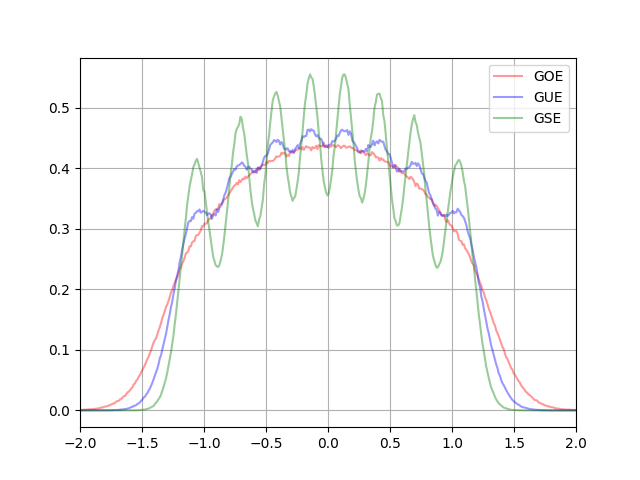
\includegraphics[width=\linewidth]{Assets/FullGaussianDensityEscaled}
		\caption{\href{https://github.com/Joao-vap/RMT-Code/blob/main/GaussianDensity.py}{GitHub - Gaussian Density} \\}
		\label{fig:a1}
	\end{subfigure}%
	\begin{subfigure}{.5\textwidth}
		\centering
		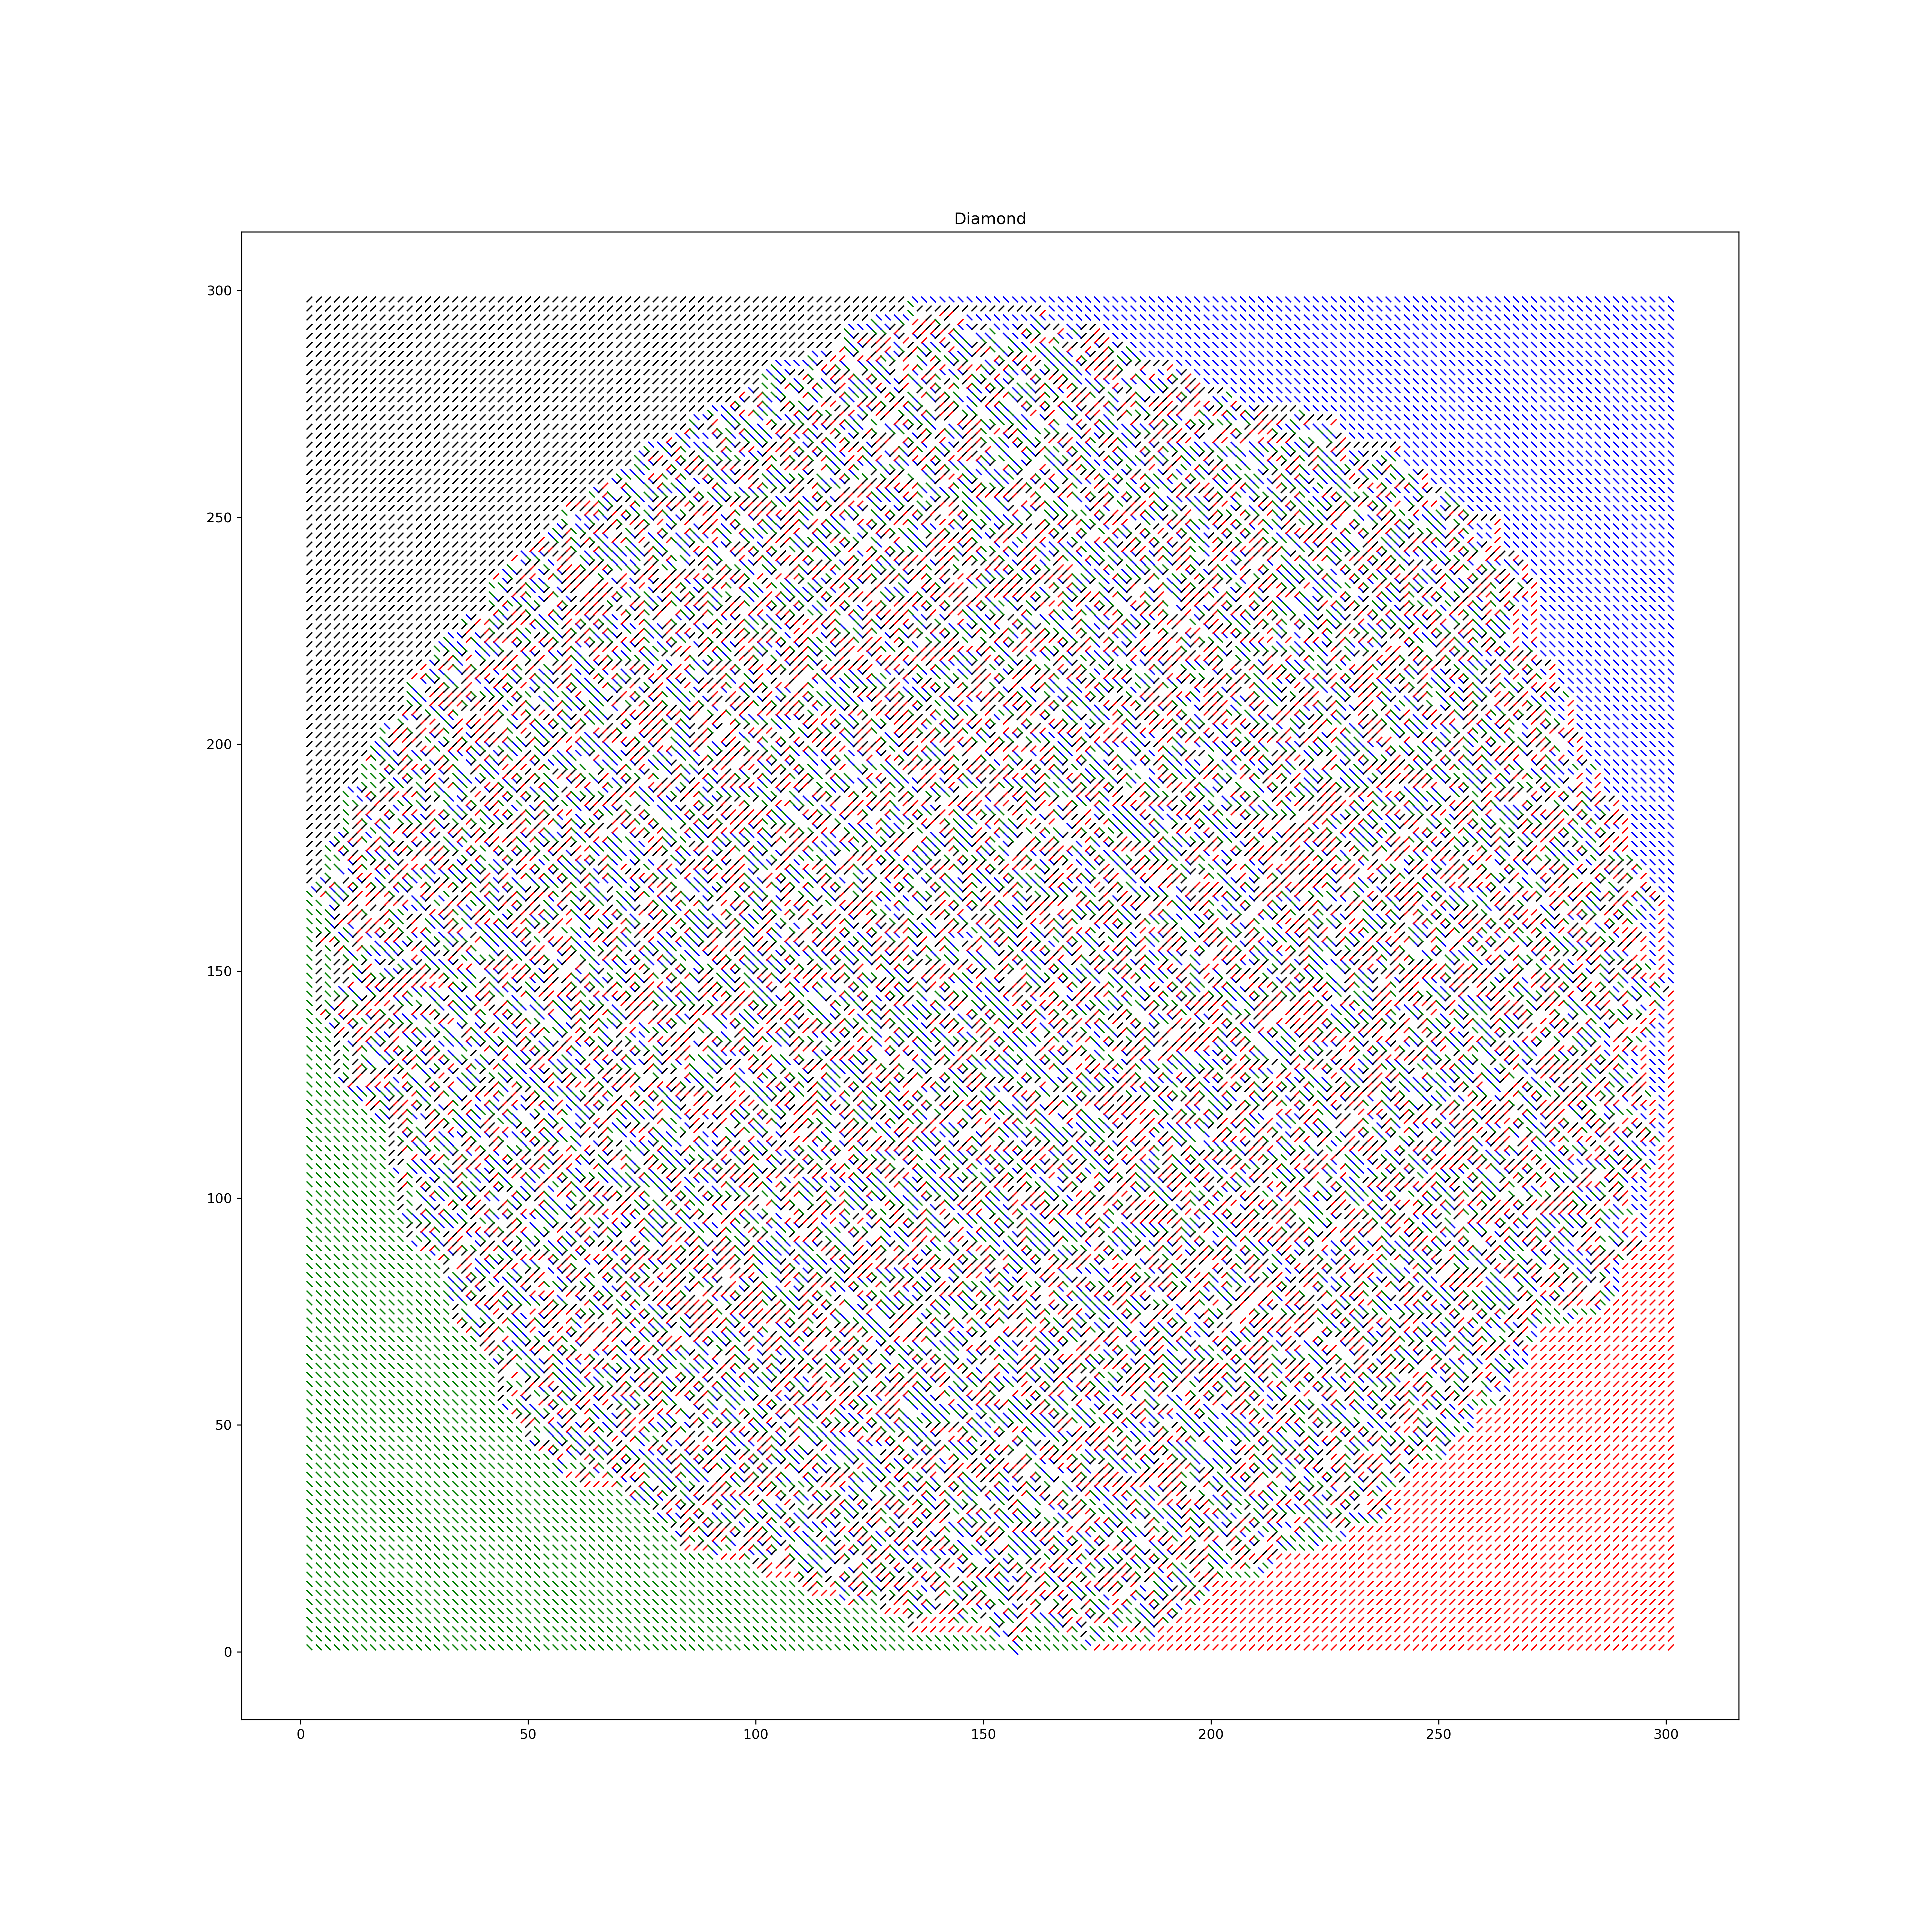
\includegraphics[width=\linewidth]{Assets/AstecDiamond}
		\caption{\href{https://github.com/Joao-vap/RMT-Code/tree/main/Tiling}{GitHub - Tiling do Círculo Ártico}}
		\label{fig:a2}
	\end{subfigure}
	\begin{subfigure}{.5\textwidth}
		\centering
		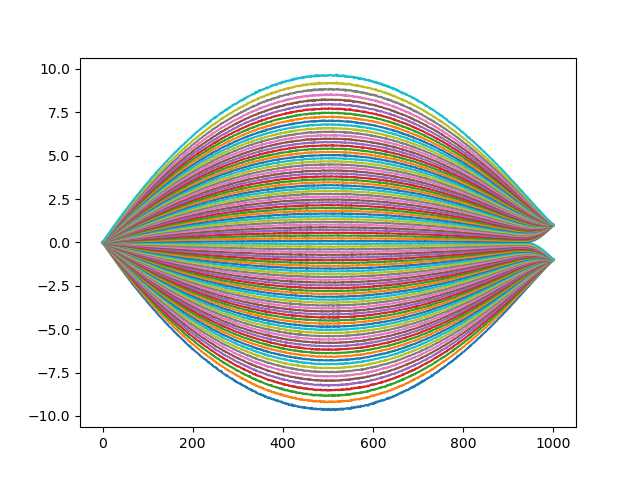
\includegraphics[width=\linewidth]{Assets/nonintersectBrownianPart-2f}
		\caption{\href{https://github.com/Joao-vap/RMT-Code/blob/main/tracywidow/N-Brownian.py}{GitHub - N Caminhos Browninanos}}
		\label{fig:a3}
	\end{subfigure}
	\begin{subfigure}{.5\textwidth}
		\centering
		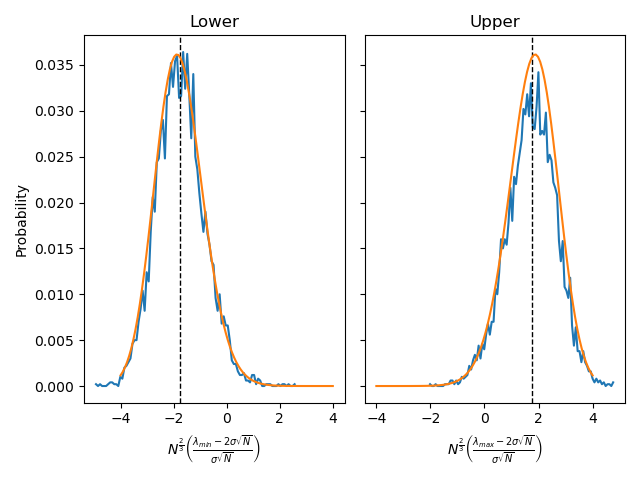
\includegraphics[width=\linewidth]{Assets/nonintersectBrownianPart-tracywidow001-distreal}
		\caption{\href{https://github.com/Joao-vap/RMT-Code/blob/main/tracywidow/TtracyWidow.py}{GitHub - Determinação da Tracy Widow}}
		\label{fig:a4}
	\end{subfigure}
	\caption{Figura \ref{fig:a1} mostra a densidade de autovalores normalizada geradas pelos emsembles de matrizes GOE, GUE, GSE para N pequeno. Figura \ref{fig:a2} é um possível tiling por dominós (peças 2x1) formando o famoso Diamante Asteca, o círculo formado é denominado Círculo Ártico e a distribuição da borda está relacionada com distribuição de autovalores máximos de emsembles especiais de matrizes. Figura \ref{fig:a3} é a representação do caminho browniano de partículas com ponto inicial determinado e $m$ pontos finais. A distribuição das partículas em cada momento é também a mesma da medida de probabilidade de autovalores do GUE. Figura \ref{fig:a4} é a validação da distribuição de borda dos caminhos brownianos que deve ser a distribuição de Tracy Widow, demonstrada na figura. }
	\label{fig:atividades}
\end{figure}

\begin{figure}
	\begin{center}
			\begin{subfigure}{.6\textwidth}
			\centering
			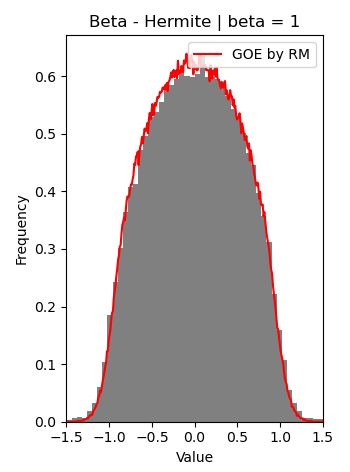
\includegraphics[width=0.7\linewidth]{Assets/b1WT}
			\caption{}
			\label{fig:art1}
		\end{subfigure}%
	\end{center}
	\begin{subfigure}{.5\textwidth}
		\centering
		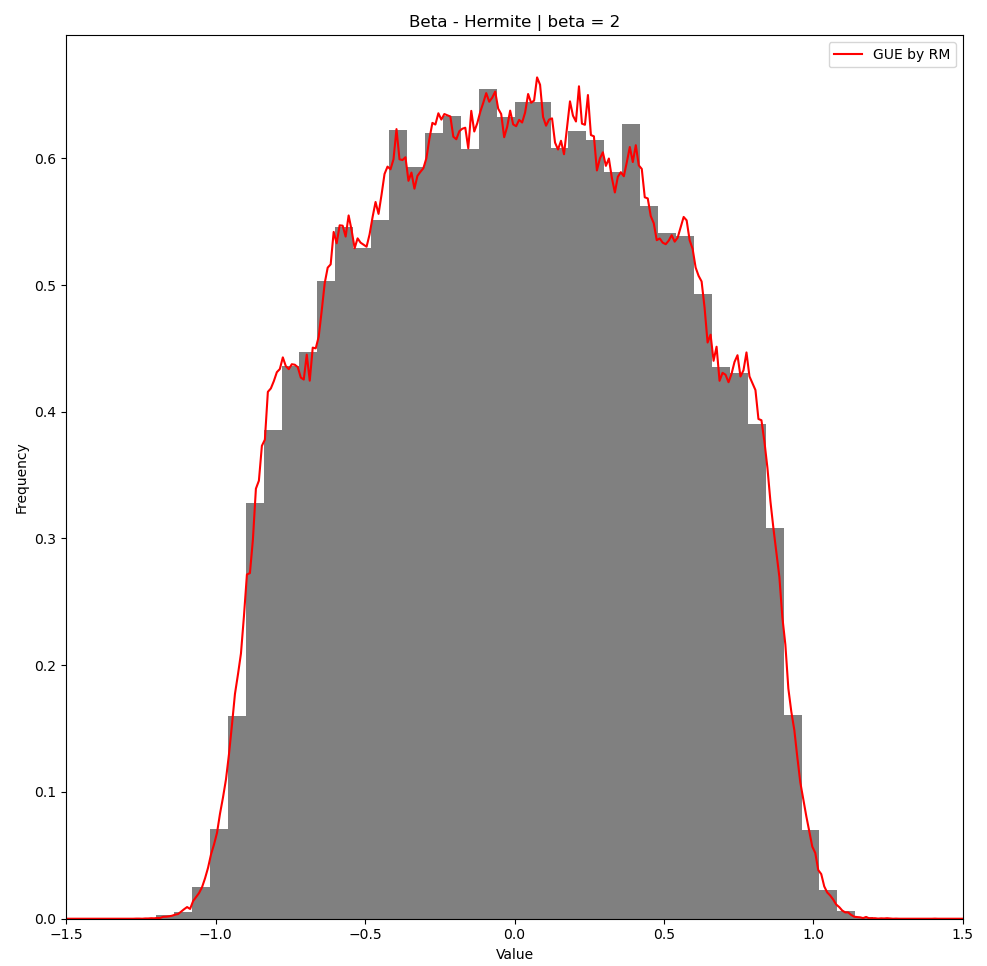
\includegraphics[width=.9\linewidth]{Assets/b2WT}
		\caption{}
		\label{fig:art2}
	\end{subfigure}
	\begin{subfigure}{.5\textwidth}
		\centering
		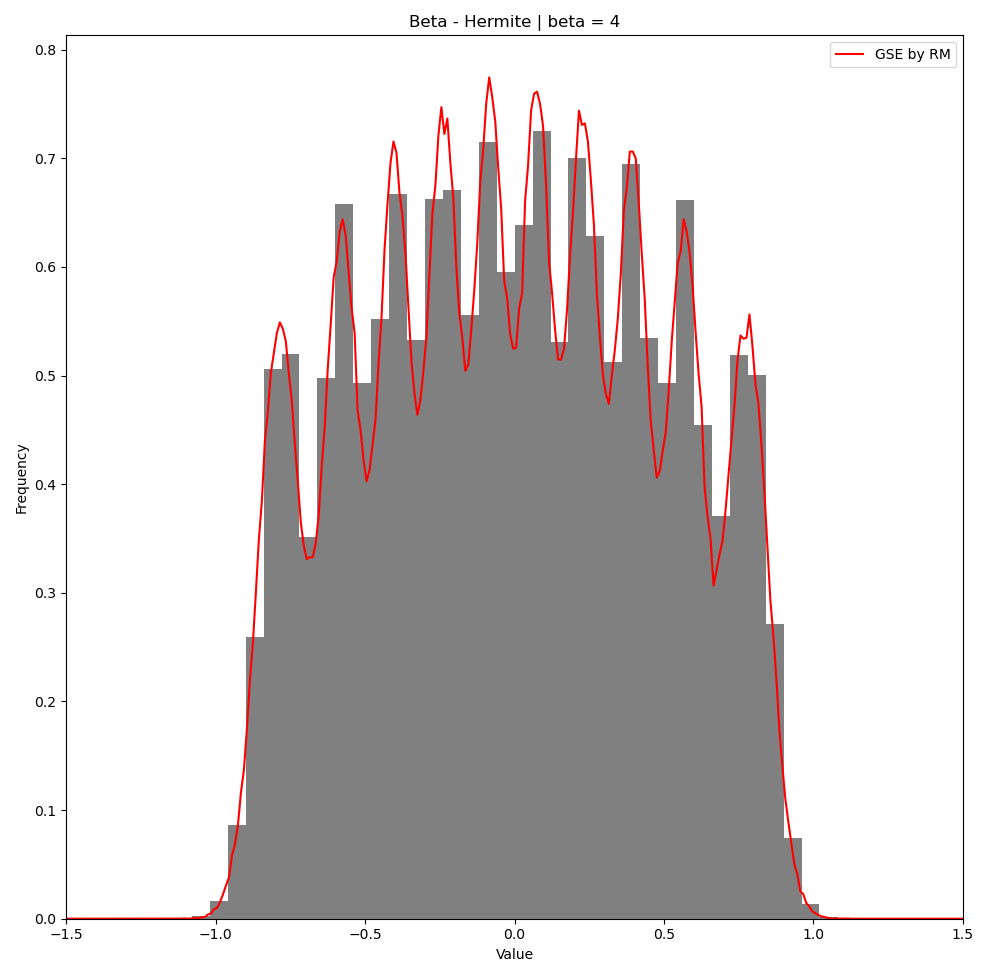
\includegraphics[width=.9\linewidth]{Assets/b4WT}
		\caption{}
		\label{fig:art3}
	\end{subfigure}
	\caption{
		As figuras representam a validação das distribuições geradas pelo algoritmo descrito no artigo \cite{Chafa__2018}. Respectivamente, nas figuras \ref{fig:art1}, \ref{fig:art2} e \ref{fig:art3} está descrito a medida obtida pela dinâmica dos pontos descrita pelo algoritmo no histograma. Em vermelho é a distribuição equivalente gerada pela mesma quantidade de observações usando modelos de matrizes aleatórios dos ensembles GOE, GUE e GSE.  O programa usado está disponível em \href{https://github.com/Joao-vap/RMT-Code/tree/main/ArticleAlg}{GitHub - Implementação do Algoritmo do Artigo}}
	\label{fig:artigo}
\end{figure}


\begin{figure}
	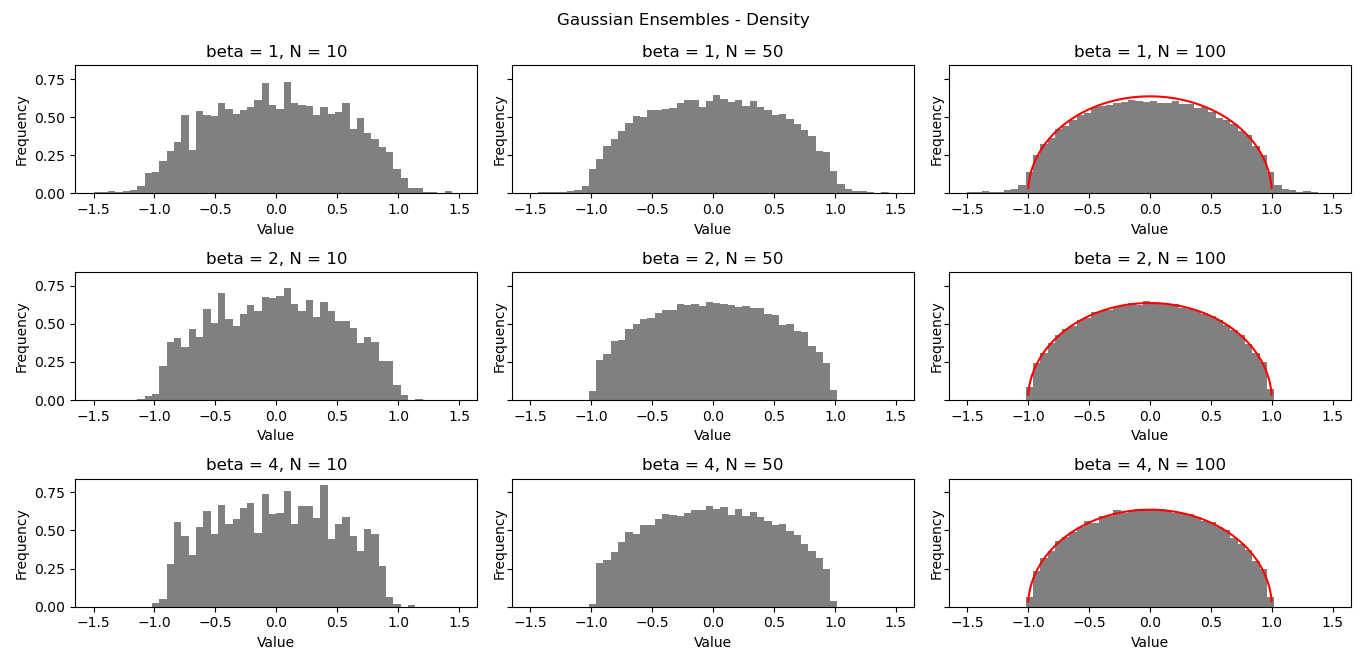
\includegraphics[scale=0.45]{Assets/validationArticleAlg}
	\caption{Validação para ensembles clássicos, utilizamos $200000$ passos registrando a cada $500$ a partir da metade dos passos. $\Delta t = 0.1$, $\gamma = 1$, $\alpha = 1.0$. Para replicar a semente foi $987991650$.}
\end{figure}


\begin{center}
	\begin{figure}
		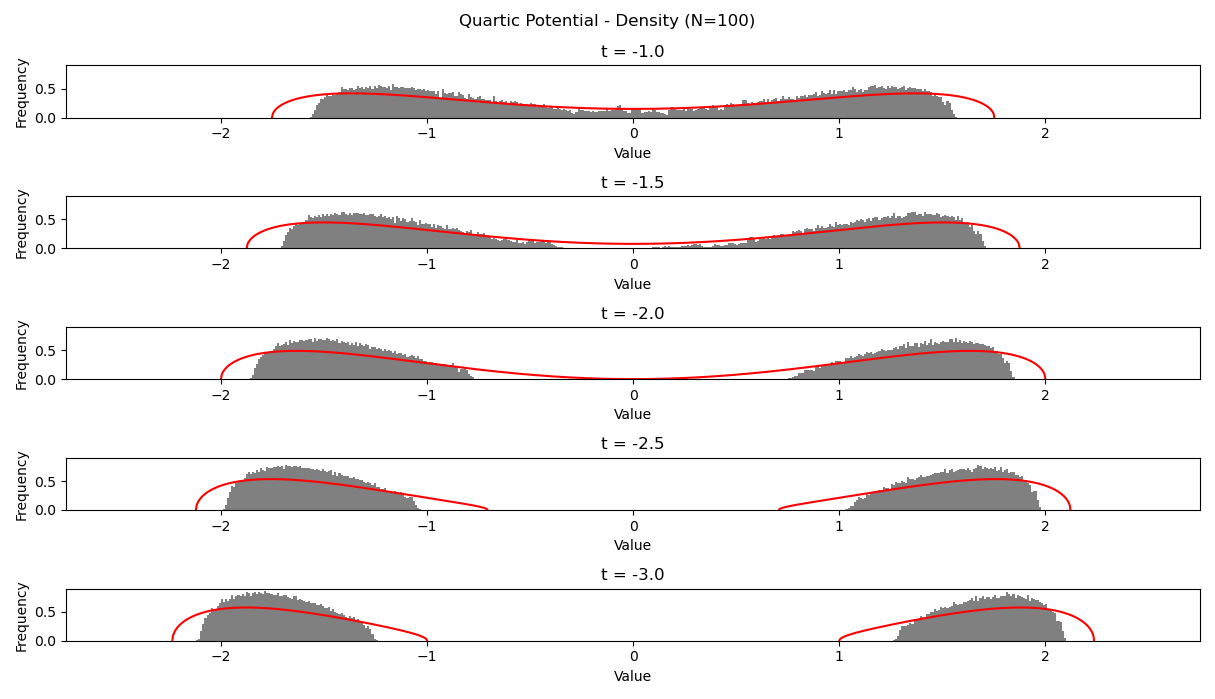
\includegraphics[scale=0.8]{Assets/validationArticleQuartic}
		\caption{Validação para potencial quártico, $V(x) = \frac{1}{4} x^4 + \frac{1}{2} x^2$. Utilizamos $1000000$ passos registrando a cada $500$ a partir da metade dos passos. $\Delta t = 0.1$, $\gamma = 10$, $\alpha = 0.1$. Para replicar a semente foi $987991650$.}
	\end{figure}
\end{center}


\begin{center}
	\begin{figure}
		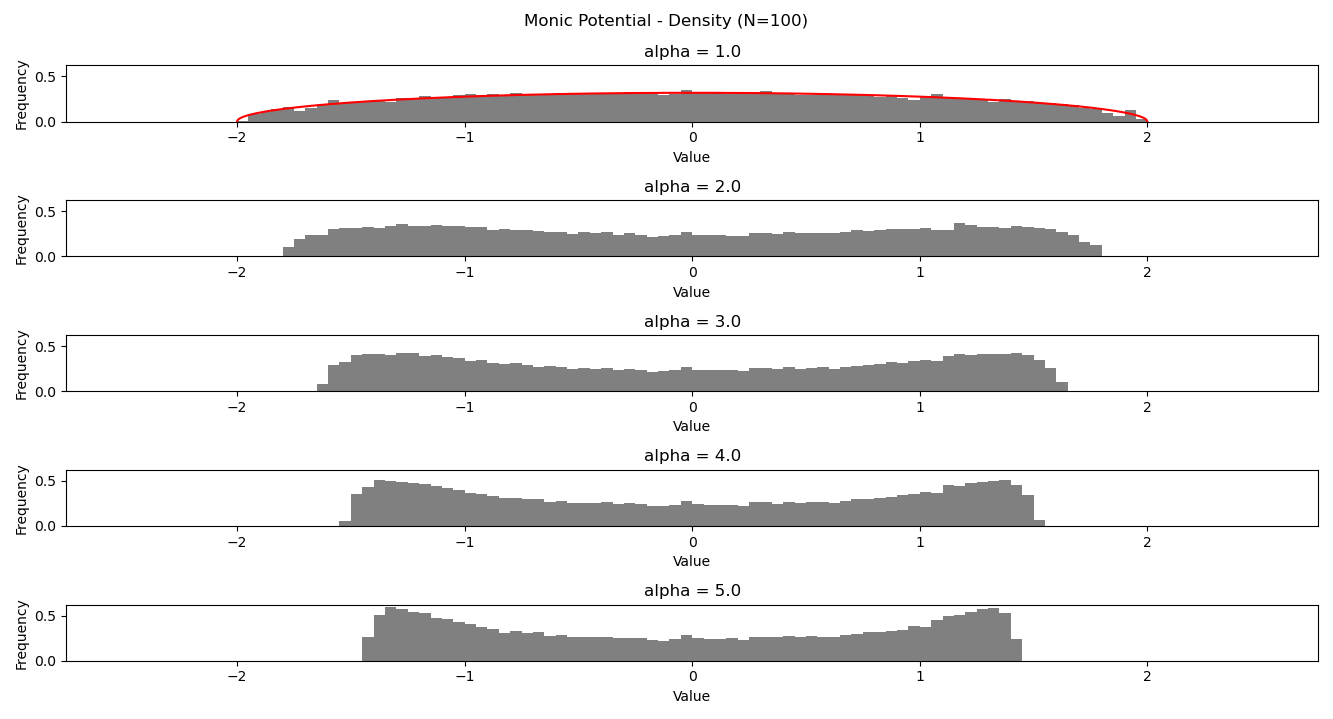
\includegraphics[scale=0.8]{Assets/validationArticleMonic}
		\caption{Validação para potencial mônico, $V(x) = \frac{t}{2 \alpha} x^{2\alpha}$. Utilizamos $1000000$ passos registrando a cada $500$ a partir da metade dos passos. $t = 1$, $\Delta t = 0.1$, $\gamma = 10$, $\alpha = 0.1$. Para replicar a semente foi $987991650$.}
	\end{figure}
\end{center}

\chapter{Plano de atividades}\label{chp:plano}

O projeto tem como base um planejamento de 12 meses, que se deram início em junho de 2023, até o momento foram realizados 5 meses de projeto.

\section{Atividades Desenvolvidas}
\label{section:atividadesdesenvolvidas}

A execução do projeto foi dividida nas seguintes etapas:

\begin{enumerate}
	\item \textbf{Revisão da Literatura em RMT, e estudo de teoria básica do GUE}, é necessário fazer vasta revisão de literatura no tema para que o aluno tenha domínio das ferramentas e métodos utilizados para o tratamento de matrizes aleatórias e suas implicações em mecânica estatística. Para isso, durante esse período será realizado o estudo da bibliografia adequada;
	
	\item \textbf{Estudo dos métodos de Simulação}, como mencionado, uma das aplicações importantes da teoria de matrizes aleatórias reside em sua conexão com gases de Coulomb. Em 2018 publicou-se o \cite{Chafa__2018}, artigo que é base para o estudo de métodos de simulação desses gases;
	
	\item \textbf{Implementação dos algoritmos}, implementa-se os métodos descritos no artigo e tenta-se estender seu uso em condições diferentes das utilizadas no artigo, como por exemplo em outros potenciais;
	
	\item \textbf{Redação dos Relatórios Científicos}, quando serão escritos os relatórios exigidos pelas normas da \textit{FAPESP}.
	
\end{enumerate}

\section{Cronograma}

Com base nas tarefas enumeradas na Seção \ref{section:atividadesdesenvolvidas}, é mostrado na Tabela \ref{tab:cronograma1ano} o cronograma atual de desenvolvimento do projeto. Em especial, os métodos de simulação puderam ser adiantados no desenvolvimento para o mês 4, previamente previsto para o mês 5 e consequentemente as implementações também puderam ser iniciadas.

%\begin{table}[ht]
%\centering
%\begin{tabular}{|c|c|c|c|c|c|c|c|c|c|c|c|c|}
%\hline
%\multirow{2}{*}{{\bf Fases}} & \multicolumn{6}{c|}{{\bf Meses}}
%\\ \cline{2-7}
%    & 1 & 2 & 3 & 4 & 5 & 6
%\\ \hline
%    {\bf 1. Revisão Literatura RMT} & x & x & x & & &  
%\\ \hline
%    {\bf 2. Métodos de Simulação} &  &  & x & x & &
%\\ \hline
%    {\bf 3. Implementação algoritmos} & & & & x & x & 
%\\ \hline
%    {\bf 4. Redação Relatórios} & & & & & & x
%\\ \hline
%\end{tabular}
%\caption{Cronograma das atividades.}
%\label{tab:cronograma6meses}
%\end{table}

\begin{table}[ht]
	\centering
	\begin{tabular}{|c|c|c|c|c|c|c|c|c|c|c|c|c|}
		\hline
		\multirow{2}{*}{{\bf Fases}} & \multicolumn{12}{c|}{{\bf Meses}}
		\\ \cline{2-13}
		& 1 & 2 & 3 & 4 & 5 & 6 & 7 & 8 & 9 & 10 & 11 & 12
		\\ \hline
		{\bf 1. Revisão Literatura RMT} & \checkmark & \checkmark & \checkmark & \checkmark & \checkmark & & & & & & &
		\\ \hline
		{\bf 2. Métodos de Simulação} &  &  &  & \checkmark & \checkmark & x & x & x & & & &
		\\ \hline
		{\bf 3. Implementação algoritmos} & & & & & \checkmark & x & x & x & x & x & x &
		\\ \hline
		{\bf 4. Redação Relatórios} & & & & \checkmark & \checkmark & & & & & & x & x 
		\\ \hline
	\end{tabular}
	\caption{Cronograma das atividades.}
	\label{tab:cronograma1ano}
\end{table}

\chapter{Participação em eventos científicos}\label{chp:particEvento}

O bolsista apresentou em dois eventos no período em que se refere o presente relatório. O Colóquio Brasileiro de Matemática (CBM) e a Semana Integrada da Física de São Carlos (SIFSC). Apenas para o primeiro, realizado no Rio de Janeiro, foi necessário o uso da reserva técnica. Por isso, segue o pôster apresentado na página que se segue. O trabalho é complementar aos estudos assintóticos e de probabilidade realizados nos meses cobertos por este relatório.

\hspace{1cm}

\hspace*{-3cm}
\begin{tabular}{|c|c|c|c|c|c|}
	\hline
	Nome do Evento & Cidade - Sede & Data & Modalidade & Apresentação & Reserva Técnica \\
	\hline
	CBM & Rio de Janeiro / IMPA & 24-28 Julho 2023 & Presencial & Pôster - Oral & Sim \\
	\hline
	SIFSC & São Carlos / IFSC-USP & 21-25 Agosto 2023 & Presencial & Pôster - Oral & Não \\
	\hline
\end{tabular}
\hspace*{-3cm}

\hspace{1cm}

O trabalho apresentado no CBM foi apresentado oralmente por meio de pôsteres no evento científico Colóquio Brasileiro de Matemática ocorrido de 24-28 de Julho no IMPA, Rio de Janeiro. Foram utilizadas duas diárias da reserva para a participação do colóquio.


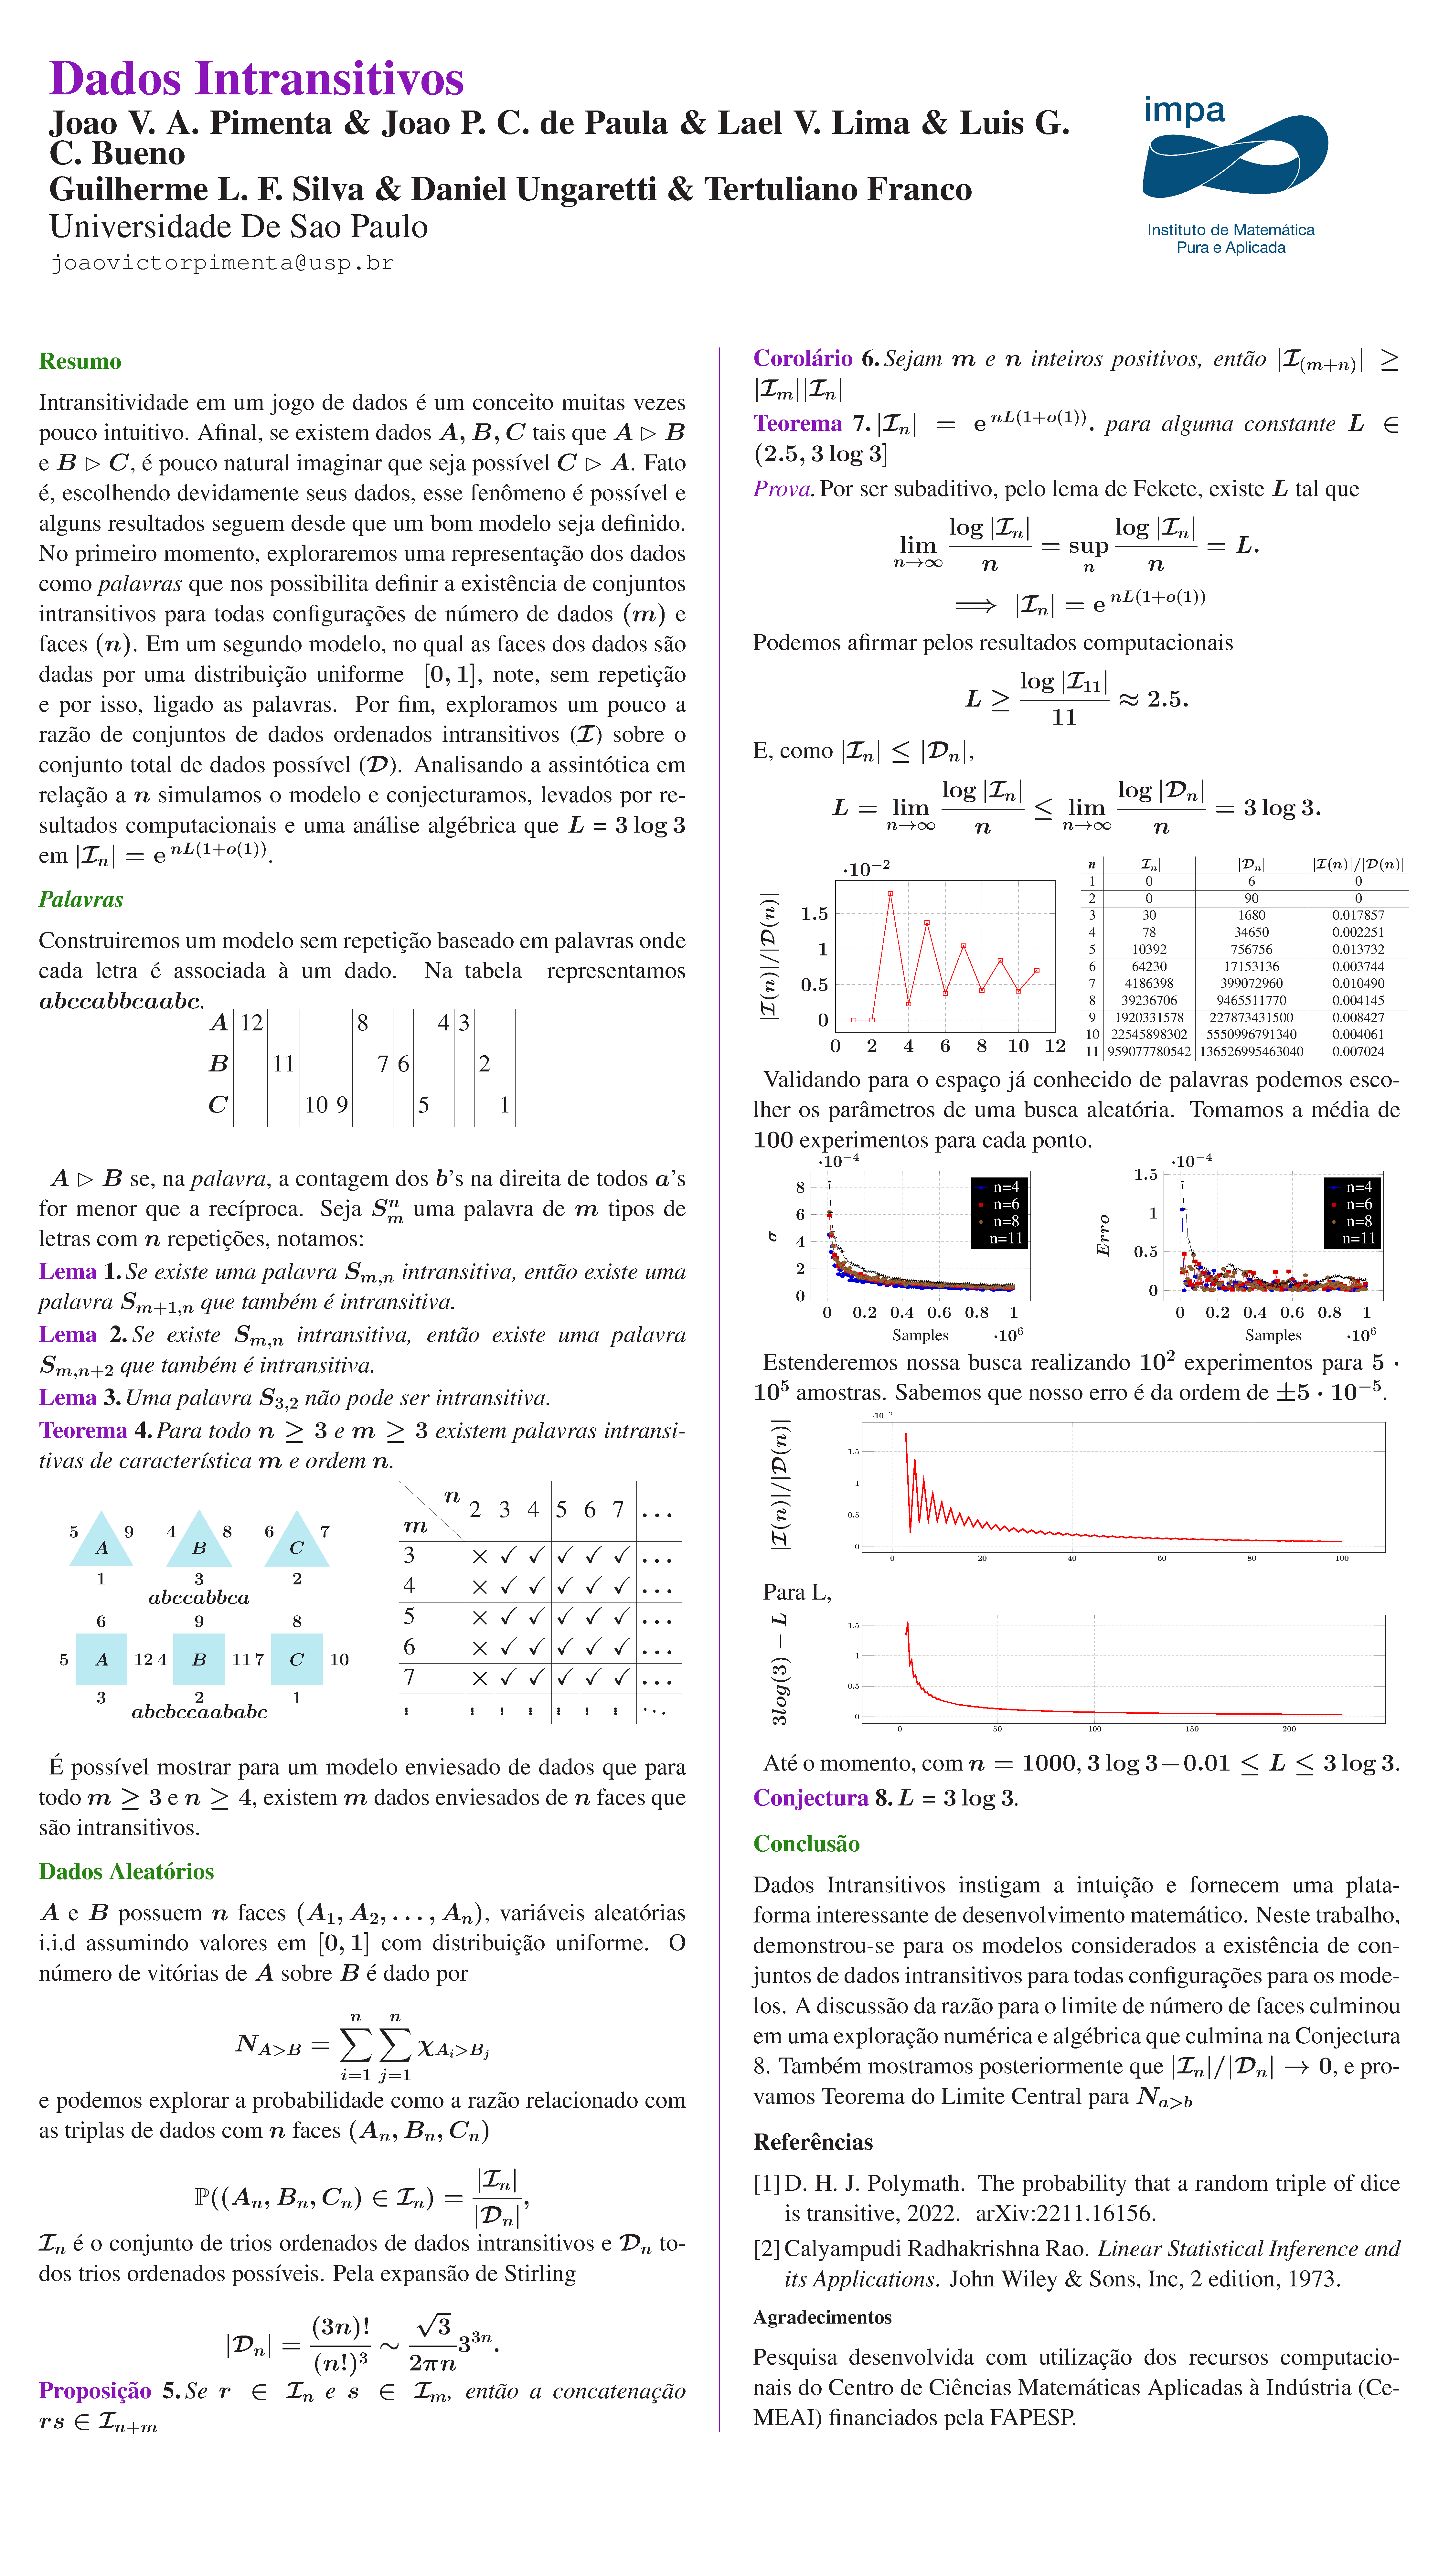
\includepdf[pages={1}]{Assets/posterwhite.pdf}

%%-----
%% Referências bibliográficas
%%-----
\addcontentsline{toc}{chapter}{\bibname}
\bibliographystyle{abntex2-num}
\bibliography{bibliografia}

%%-----
%% Fim do documento
%%-----

%\appendix
%\chapter{Implementação Algoritmo}

%\inputminted[
%frame=lines,
%framesep=2mm,
%baselinestretch=1.2,
%bgcolor=white,
%fontsize=\footnotesize,
%linenos
%]{FORTRAN}{Assets/HKMC.f}

\end{document}